\chapter{Conclusion}
In this thesis defense, a method to estimate the thickness and to refine the trajectory of a ribbon-like feature in \ac{VHR} aeral orthoimagery has been presented. 
We were able to obtain both high qualitative and quantitative results for segmenting walking paths in aerial imagery by refining \ac{OSM} features. The method is fast, and has only a few parameters with clear interpretations.
The proposed approach does not rely on extensive training on annotated data, but instead learns to fit the underlying imagery based on a trimap that is specified by parameters $\MinRadius{}, \MaxRadius{}, \MaxDistance{}$ which values that are easily determined based on the task, and are unlikely to require adjustment. 

We evaluated this work by comparing it mainly to approaches for interactive image segmentation. 
Because most automatic approaches for extracting street-maps focus on extracting coarse trajectories (which we take as input) rather than on precise alignment and width estimation. 
We focused on modeling footways which are small, thin, easily occluded, and often modified due to construction.
We believe that this approach is a natural tool to improve segmentation by post-processing automatically extracted street networks, and also by enabling fast interactive annotation of aerial images by refining hand-entered paths such as those found in \ac{OSM}.

\section{Summary}
Chapter 2 introduces a few important background knowledge for better understanding of this thesis defense. We go through \ac{VHR}, \ac{OSM}\cite{OpenStreetMap}, \ac{CRF}\cite{MAL-013}, \ac{GMM}\cite{sridharan2014gaussian} and \ac{DP}\cite{bellman2013dynamic} to understand the basic of our approach.   

Chapter 3 shows the experiments that we researched on similar topics on feature extraction from image and sidewalk segmentation method. Mainly, we compared with segmentation tools, such as grabcut\cite{Rother2004-ou}, slic\cite{Achanta:149300}, and active contours \cite{Kass88snakes:active}. These three methods had fairly performance on segmentation sidewalk feature from input. Different but related methods were also applied such as road extraction\cite{road_detect}.

Chapter 4 carefully considers a hypothesis for our dynamic programming approach. Introduce the idea to segment ribbon-like feature by converting it's original shape into ribbon-shape. Also we developed a mathematics solution and a lattice representation of the problem, to help us build our dynamic programming solution better in the chapter 6.

Chapter 5 shows the publication that submitted base on our approach. We reproduce the hypothesis with more detail demonstration for the approach and involved algorithms. 

Chapter 6 brings a four-step approach in order to generate precise boundaries for given sidewalk, locate sidewalk geometric information, generating ribbon-image, applying density estimation function and applying our dynamic program algorithm with width control. Output from the approach would be compared from the other methods.

\section{Failure Cases}

We produce some failure cases to show what we need to improve for the future work. 

\begin{enumerate}
    \item Miss matching data set: Figure \ref{fig:oxford_fail_1} shows the failure case when the input map data and the trajectory data not match. The map data is older than the trajectory data, so the boundaries we generated is not yet existed on the map. Since the road structures changes over time, it's possible to get the data set in different time stamp. 
    \item Irregular Intersections: Figure \ref{fig:oxford_fail_2} shows the failure case when process irregular shape intersections. Our approach is able to generate the boundaries when the sidewalk is able to reshape into ribbon-image. Such as in figure \ref{fig:oxford_fail_2}, it's not yet able to produce the sidewalk boundaries with irregular shape intersection.
    \item Fully blocked sidewalk: \figref{fig:ny_fail_1} shows sample of sidewalks that fully blocked by obstacles, tree crown in our case. Base on the initial trajectory we find from open source, there must be a sidewalk under the tree crown. We count this as 'failure' cases since it's impossible for us to determine the accuracy for our result. 
\end{enumerate}

\begin{figure}
    \centering
    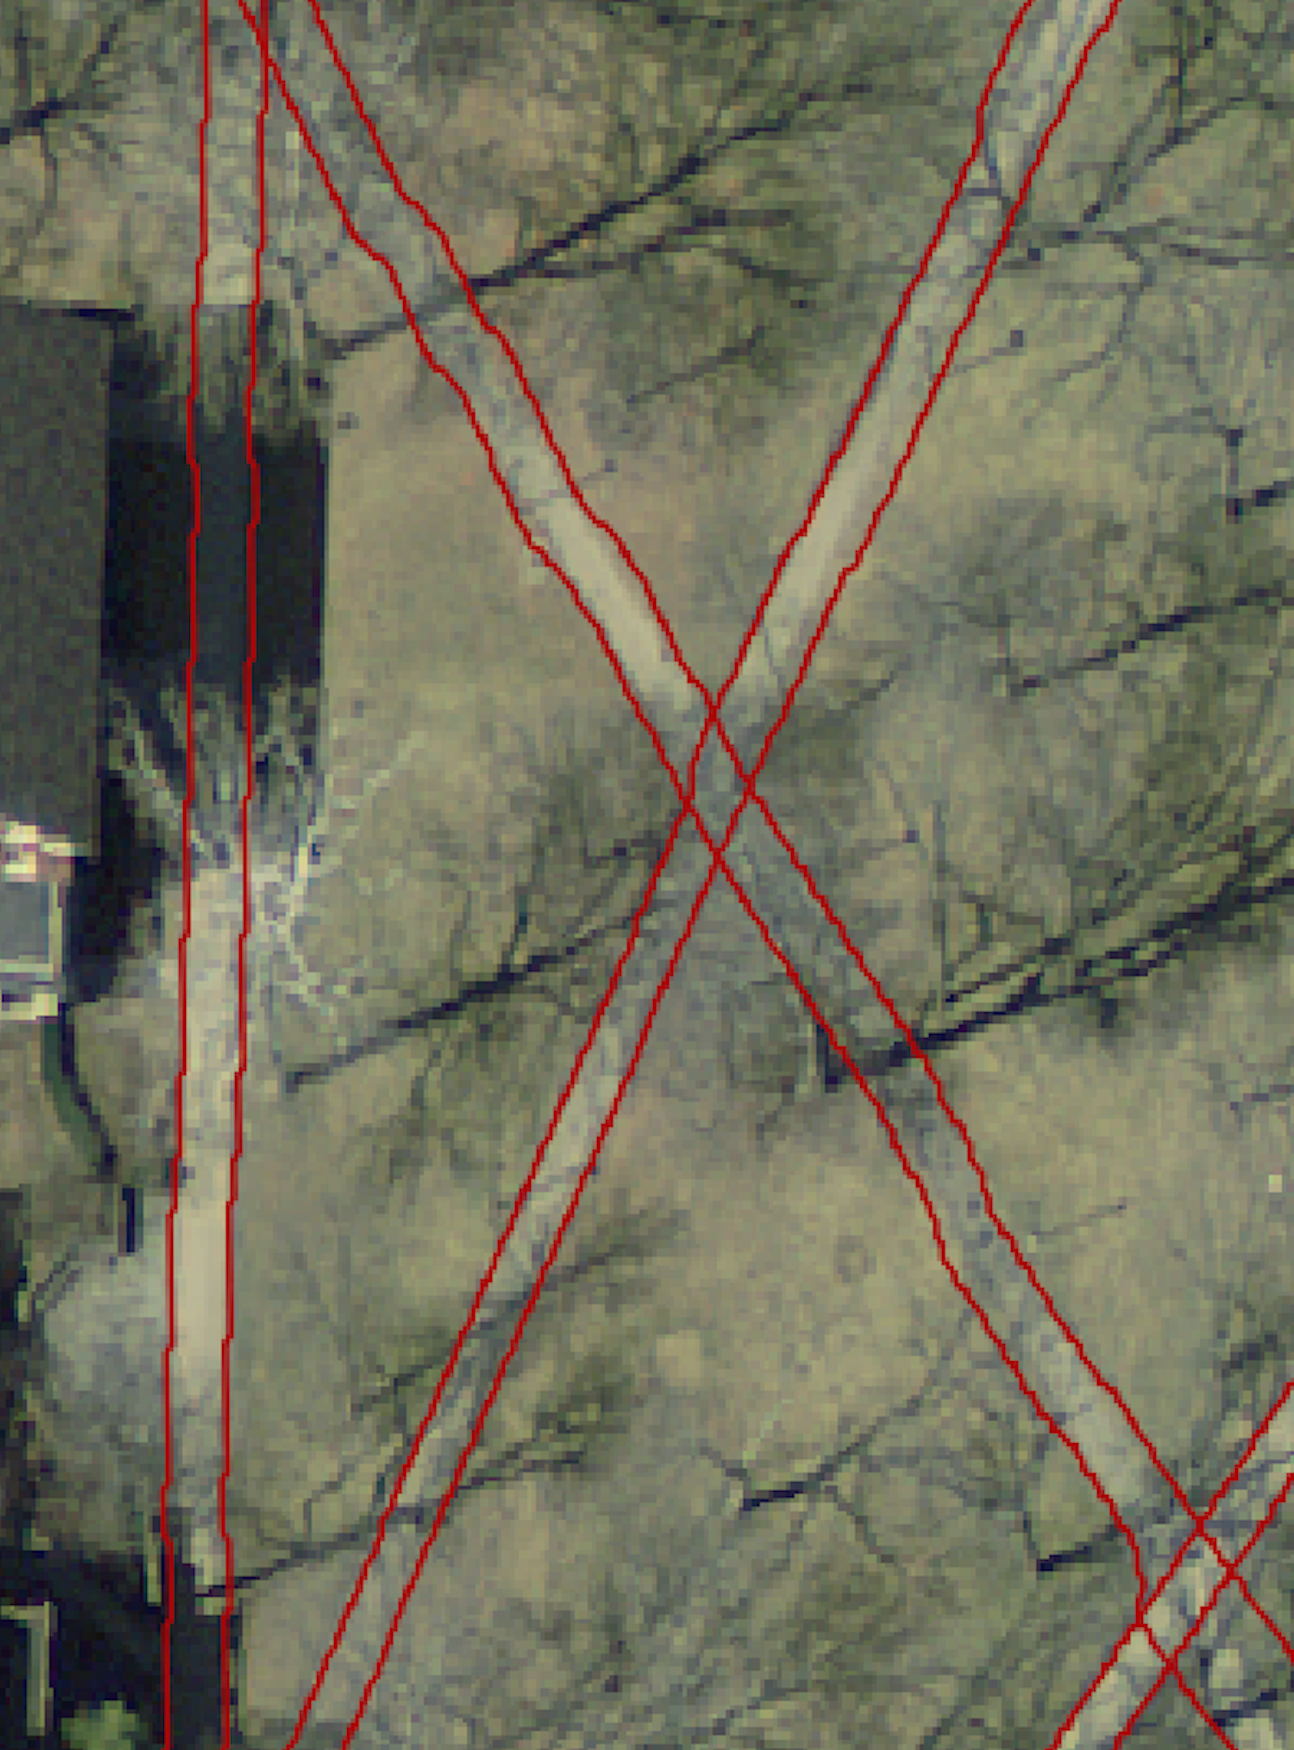
\includegraphics[width=0.83\textwidth]{Figures/oxford_fail_1.png}
    \caption[Failure Case 1]{Demonstration on failure cases. Due to the fact that road structures may change overtime. It's possible to produce the output with the input map and the initial trajectory within different time stamp. Sample figure shows our approach produce 'incorrect' sidewalk boundaries because the map data is older than the trajectory so we are producing the sidewalk that were not built yet.}
    \label{fig:oxford_fail_1}
\end{figure} 

\begin{figure}
    \centering
    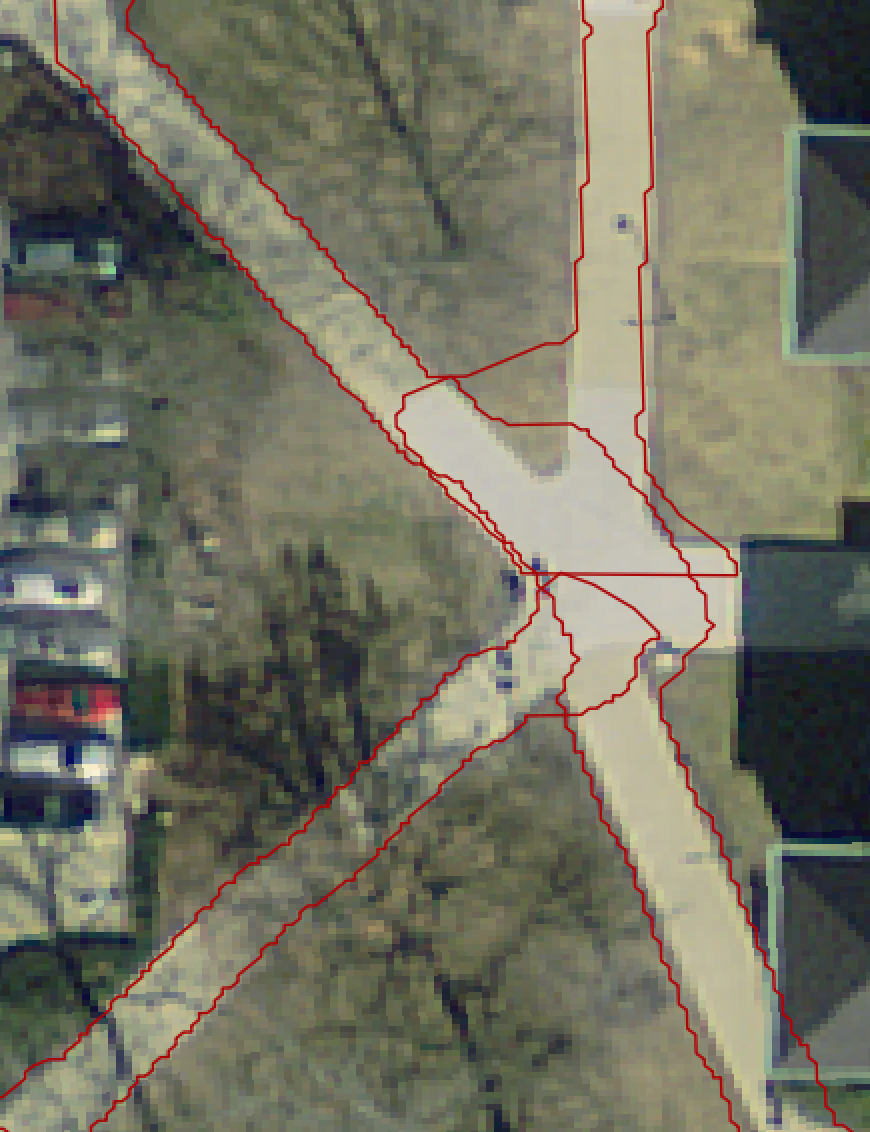
\includegraphics[width=0.9\textwidth]{Figures/oxford_fail_2.png}
    \caption[Failure Case 2]{Demonstration on failure cases. Our approach was developed to produce boundaries for single sidewalk, and it's not yet able to process intersection with irregular shape.}
    \label{fig:oxford_fail_2}
\end{figure} 

\begin{figure}
    \centering
    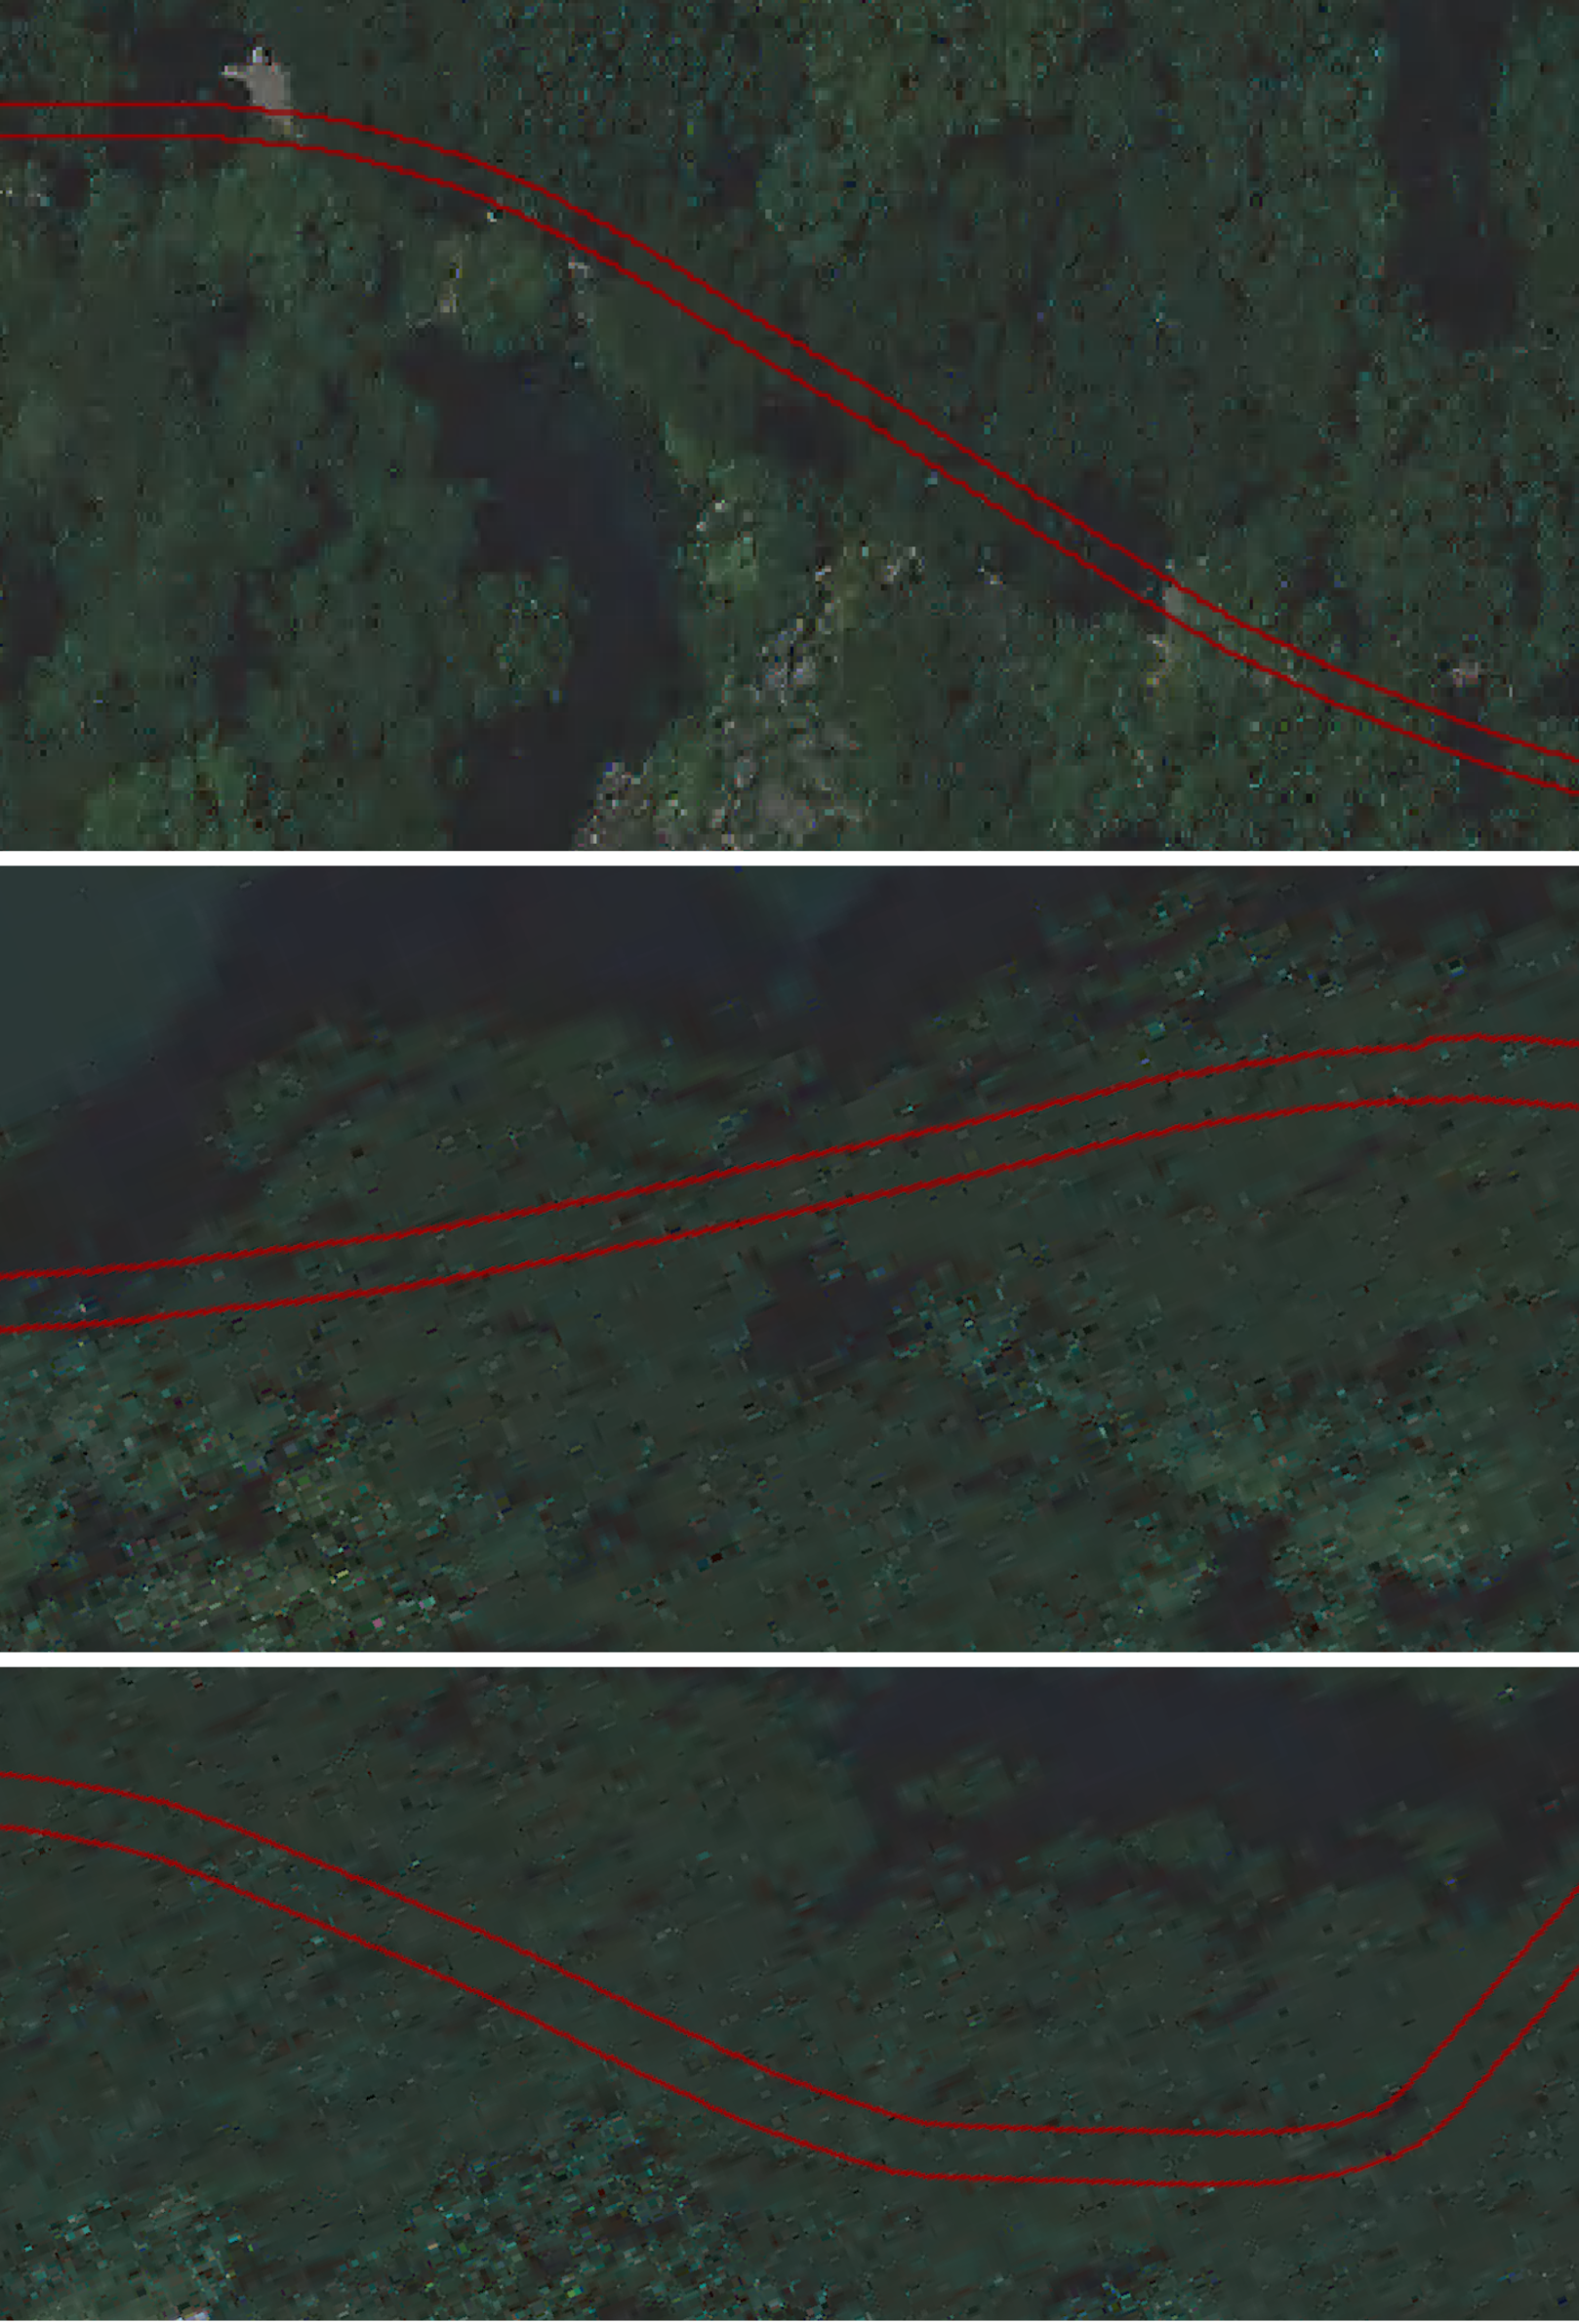
\includegraphics[width=0.8\textwidth]{Figures/ny_failcase.png}
    \caption[Failure Case 3]{Demonstration on failure cases. Our approach is not able to determine the sidewalk boundaries that's completely blocked by obstacles. The result is base on the average of sidewalks width but it's impossible for us to compare the prediction with accurate result.}
    \label{fig:ny_fail_1}
\end{figure} 

\section{Future Work}

There's couple more ideas we would like to attempt.

\begin{enumerate}
    \item To simplify the process, we would like to generate the sidewalk with just latitudes and longitudes.
    
    we can use the latitudes and longitudes data to locate a part of a map via Overpass Turbo \cite{overpass_turbo}, it supports features such as sidewalks geometric location since it's connecting with the database from \ac{OSM} \cite{OpenStreetMap}. Also, with the input latitudes and longitudes data, we can extract the map with given range from Google map or other open map source. Then just simply pass in both data set with our approach to generate whole sidewalk information for the whole site. 
    
    \item We'll give hypothesis to process the intersection area. By identify the point that is overlapped as intersection part (same node in multiple ways), we connect nodes on each way that are adjacent to the point. By extend each path a little bit more into the adjacent path to finish the intersection.
    
\end{enumerate}